\documentclass{standalone}
\usepackage{tikz}
\begin{document}
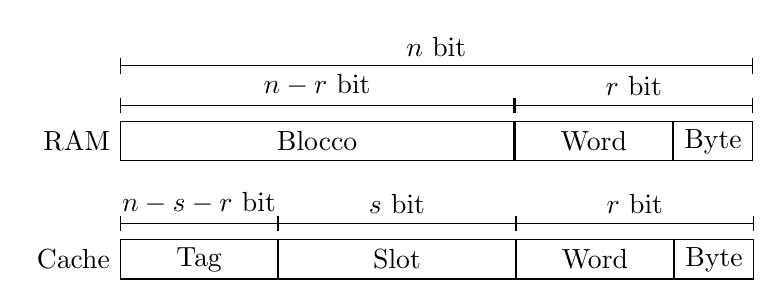
\begin{tikzpicture}
    \draw
    
    (0,0)node[rectangle,draw,minimum height=0.5cm,minimum width=5cm,anchor=west](addr){Blocco}
    (addr.east)node[rectangle,draw, minimum height=0.5cm,minimum width=2cm, anchor=west](w){Word}
    (w.east)node[rectangle,draw, minimum height=0.5cm,minimum width=1cm,anchor=west, inner sep=0](b){Byte}
    (addr.west)node[left]{RAM}    

    (0,-1.5)node[rectangle,draw,minimum height=0.5cm,minimum width=2cm, inner sep=0,anchor=west](tag){Tag}
    (tag.east)node[rectangle,draw, minimum height=0.5cm,minimum width=3cm, anchor=west](addr1){Slot}
    (addr1.east)node[rectangle,draw, minimum height=0.5cm,minimum width=2cm, anchor=west](w1){Word}
    (w1.east)node[rectangle,draw, minimum height=0.5cm,minimum width=1cm,anchor=west, inner sep=0](B){Byte}
    
    (tag.west)node[left]{Cache}
    (addr.north west)++(0,0.2)coordinate(a1)
    (addr.north east)++(0,0.2)coordinate(a2)
    (b.north east)++(0,0.2)coordinate(a3)

    (addr.north west)++(0,0.7)coordinate(a4)
    (b.north east)++(0,0.7)coordinate(a5)
    
    
    (tag.north west)++(0,0.2)coordinate(b1)
    (tag.north east)++(0,0.2)coordinate(b2)
    (addr1.north east)++(0,0.2)coordinate(b3)
    (B.north east)++(0,0.2)coordinate(b4)

    ;
    \draw[|-|](a1)--(a2)node[midway, above]{$n-r$ bit};
    \draw[|-|](a2)--(a3)node[midway, above]{$r$ bit};
    \draw[|-|](a4)--(a5)node[midway, above]{$n$ bit};

    
    \draw[|-|](b1)--(b2)node[midway, above]{$n-s-r$ bit};
    \draw[|-|](b2)--(b3)node[midway, above]{$s$ bit};
    \draw[|-|](b3)--(b4)node[midway, above]{$r$ bit};
    
    
\end{tikzpicture}
\end{document}